% vim: set tw=78 sts=2 sw=2 ts=8 aw et ai:

The solution I used for SourceDotCode involves a Supervisor process, which will monitor the execution of a program, and terminate its execution when encountering certain "dangerous" system calls.

Examples of such system calls are:
\begin{enumerate}
\item{sys_reboot}
\item{sys_socketcall}
\item{sys_clone}
\item{sys_unlink}
\end{enumerate}

The Linux Kernel provides ptrace, a consistent interface to implement this feature, which is commonly used by debugging software like gdb, or strace.
The supervisor process will make use of the ptrace system call to monitor the execution of the main program, as we can see in [fig1].

\begin{figure}
\begin{center}
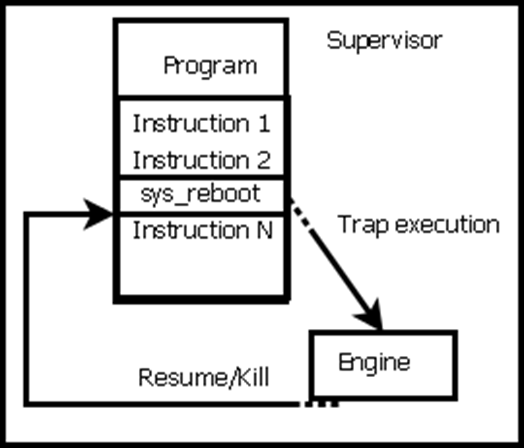
\includegraphics[scale=0.5]{pics/superv.png}
\caption{Supervisor model}
\end{center}
\label{fig1:superv}
\end{figure}

The complete architecture of the service is shown in [fig2].
There will be a Web Service Client, which sends requests to the Web Server in the form of JSON messages.
The Web Server will receive the requests, and dispatch them to a Build Agent entity.

The Build Agent will be responsible with providing the runtime execution environment for the program.
It will instantiate one Supervisor process for each program run, and then it will return the result to the Web Server.
Then, the Web Server will return the result to the user.

From a performance point of view it's critical that the communication between the Web Server and Build Agent be as smooth as possible.
Therefore, the Build Agent should be implemented using asynchronous I/O.

\begin{figure}
\begin{center}
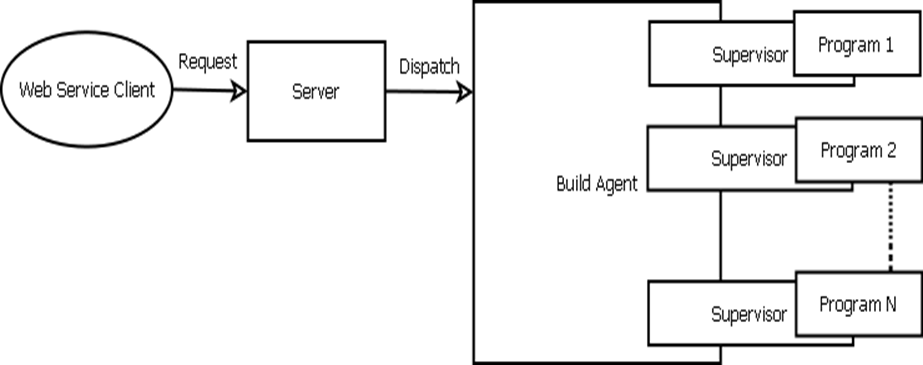
\includegraphics[scale=0.3]{pics/arch.png}
\caption{Arch model}
\end{center}
\label{fig2:arch}
\end{figure}
